
\chapter{Machine Learning}

The general idea behind machine learning is this: Given a set of data, a machine creates a model that can be used to predict relationships between the various datum. The reasons for using a machine is generally because the size of the dataset, as well as the necessary computational requirements needed to make these models, is well beyond what is reasonable for a human to do alone.

Machine learning breaks down each element of a dataset into a set of \textbf{features} which describe it and differentiate it from the other elements. The resultant model is a collection of \textbf{parameters} that describe the relationship between elements of the dataset. \textbf{Hyperparameters} are parameters used in running the algorithm which arrives at the aforementioned parameters, and are not considered parameters of the model themselves.

Most of machine learning can be broken up into three general sub-disciplines:
\begin{itemize}
	\item \B{Supervised Learning}: takes a set of labelled feature vectors and builds a model to predict unlabelled data. Simple linear regression is an example of supervised learning.
	\item \B{Unsupervised Learning}: takes a set of unlabelled feature vectors. This type of learning is useful for things like clustering, here the model looks to pair like-with-like, or dimensionality reduction, where the model translates a large set of features into a smaller set.
	\item \B{Reinforcement Learning}: uses a set of feature vectors to approximate a state which it can interact with through a set of actions, each of which are chosen to try to maximize some numerical reward signal. 
\end{itemize}



In general, any machine learning algorithm can be broken down into three components \cite{burkov}
\begin{itemize}
    \item A loss function (e.g. least squares)
    \item An optimization criterion based on the loss function (e.g. the loss landscape is convex); and
    \item An optimization routine leveraging training data to find a solution to the optimization criterion (e.g. gradient descent)
\end{itemize}

\subsection{Hyperparameters}

Hyperparameters are not optimized via the machine learning algorithm itself and instead are configured by the data analyst. One method to find a good set is \B{grid search} which combinatorically scans over each parameter (typically in log scale). This of course doesn't work too well when the number of hyperparameters in your model grows. 

\B{Random search} uses a statistical distribution for each hyperparameter which each get sampled from when making a new model to test.

\B{Bayesian hyperparemeter optimization} uses past evaluation results to choose the next values to evaluate. This aims to minimize the number of expensive optimizations you have to do.





\section{Support Vector Machines}\label{sub:svm}
Support Vector Machines (SVM) classify data-points by drawing boundaries between them. These boundaries are called ``Hyperplanes" and slice the points in their feature vectors. The technical definition of a hyperplane is any flat affine subspace. The data points “support" the each of these planes. i.e those closest to each plane are optimized around. In the case of two classes $y_i \in {-1,1}$. The ideal plane is defined as
\begin{align}
		\B{wx}_i-b =0
\end{align}
Where $\B{w}$ is the weights vector, which is optimized for, $\B{x}_i$ is the feature vector, and $b$ is the offset. This plane separates the two classes based off of the sign of any feature vector put into this equation
\begin{align}
	y = \textrm{sign}(\B{wx}_i-b)
\end{align}
One should class should give positive values, and the other, negative values. Mathematically we look for each point to obey

\begin{align}
	\B{wx}_i-b &\ge +1 ~\textrm{if}~ y_i = +1.  \label{svm_planes_pos}\\
	\B{wx}_i-b &\le -1 ~\textrm{if}~ y_i = -1.  \label{svm_planes_neg}
\end{align}

The above equations define planes as shown in Figure \ref{fig:svm}. The closest points of either classes are a separated by a distance $2/ ||\B{w}||$. We want the plane to be maximally discriminating, which is equivalent to maximizing this distance, or equivalently, \emph{minimizing} $||\B{w}||$. Using quadratic programming optimization we typically look to minimize \cite{burkov}


\begin{align}\label{svm_loss}
||\B{w}||^2
\end{align}

SVMs that minimize this function are said to have \emph{hard-margin}s, since points that fall on the wrong side of the hyperplane are not considered in the minimization procedure. 

\begin{figure}
\centerline{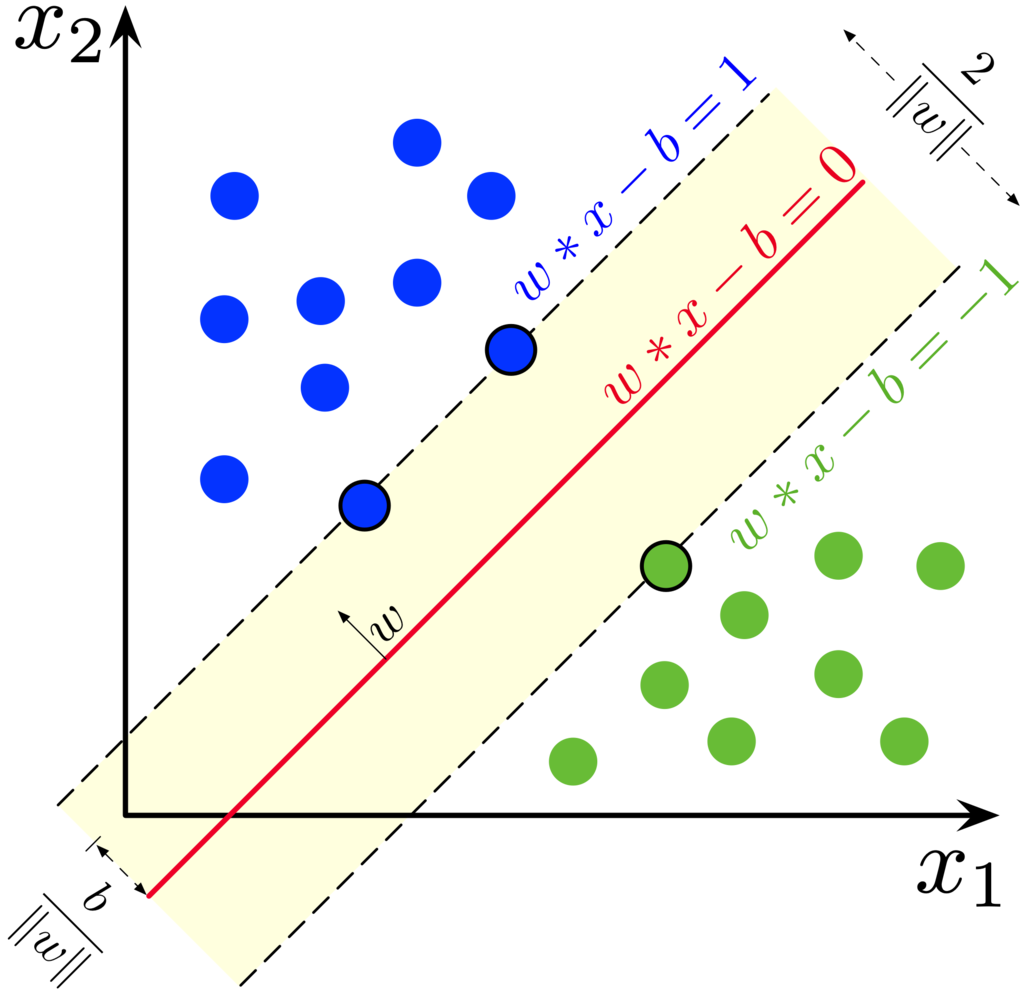
\includegraphics[width=0.5\linewidth]{mathematics/fig/svm.png}}
\caption{Maximum-margin hyperplane for an SVM trained with two classes \cite{wiki_svm}}
\label{fig:svm}
\end{figure}

\subsection{Hinge Loss}

If the classes are not cleanly distinguishable, which can happen if there is noise in the data, or the classes aren't entirely separable, one can look to minimize the \textbf{hinge loss function}, defined as
\begin{align}\label{hinge}
	C||\B{w}||^2 + \frac{1}{N}\sum_{i=1}^N \max(0,1-y_i(\B{wx}_i-b))
\end{align}
The first term in Equation \ref{hinge} is proportional to \ref{svm_loss}, while the second term is related to components on the wrong side of the boundary. Looking at Equations \ref{svm_planes_pos} and \ref{svm_planes_neg}, we see they are equivalent to 
\begin{align}
	y_i(\B{wx}_i-b) -1\ge 0\rightarrow 1- y_i(\B{wx}_i-b) \le 0
\end{align}
Therefore for any points on the correct side of the boundary, this expression is negative and $0$ is taken from the $\max$ function. However, if the point is on the \emph{wrong} side of the hyperplane, the loss function then has an added term proportional to how far away it is from the decision boundary.

SVMs that minimize the hinge loss are considered \emph{soft-margin}, since they allow for points fo fall on either side.

The choice of $C$ determines how much relative weight to give to the margin size (first term) and mislabelling (second term). A large $C$ gives a large margin which is good for generalizing the problem, while a small $C$  looks to classify the training data well.

\section{Decision Trees}
A decision tree is an acyclic graph that can be used to make decisions. Each ``leaf" of the tree assigns a label to the given feature vector. A balanced decision tree is one for which the questions split the groups into equal parts.

\subsection{Entropy}
Given $N$ different possible labels a feature vector could be associated to, we define $p_i$ with $i\in (1,N)$ as the proportion of any given label $i$. Using our full training dataset $D$, we can then define the entropy $S$ of the model as 

\begin{align}
	S^{(D)} = -\sum_{i=1}^N p^{(D)}_i\ln p^{(D)}_i
\end{align}

This tells us roughly how mixed up our dataset is. If the training data has two labels which are equally populated in the dataset, we have correspondingly larger energy than if we had only one of the labels show up. In the ideal case, each leaf of a decision tree will have just one label. A metric by which we can gauge how close we are to this ideal is by \emph{minimizing the entropy} of our model. 

There are a number of algorithms that that recursively split the dataset into those with smaller entropy i.e. $D\rightarrow D_1, D_2$. After doing this the effective entropy among the two independent datasets can be remeasured and compared with that before the split. This can then continue until a number of conditions are met such as you have only one kind of label, or there are no more splits that could further reduce the entropy.

\subsection{Boosted Decision Trees}
TODO
\subsection{Random Forests}
TODO
\subsection{Bootstrap Aggregation}
TODO


\section{Training Models}


\subsection{Linear Regression}
Linear regression is a model which presumes a linear relationship between the feature vectors $\B{x}$ and their corresponding label $y$. The linear model is defined as

\begin{align}
    y_i = \B{wx}_i +b
\end{align}
Where the index $i\in(1,N)$ denotes the specific data point of the $N$ you are considering. The typical \B{error function} $\mathcal{E}$ (sometimes called a loss function) that is used is \B{sum of squared error} (SSE) which is written as
\begin{align}
    	\min_\B{w}\sum_{i=1}^N\Big(\B{wx}_i +b - y_i\Big)^2
\end{align}

Which is read as a minimization of the expression with respect to the weights $\B{w}$. 


\subsubsection{Exact Solution}\label{lin-reg-exact}
The sum of squared error (SSE) loss function is preferred in part because it is differentiable, which allows for an exact solution. We can take as an example a dataset with $i\in(1,N)$ which includes one feature $x_i$ and its corresponding label $y_i$. This linear model is defined as

\begin{align}
y_i = wx_i + b
\end{align}

Now we wish to minimize our loss function. We can then recall that a function is at its extremum (here minimum) when the derivative is zero. Therefore we take the derivative with respect to both of the weights. For $w$ we have
\begin{align}
\frac{\partial \mathcal{E}}{\partial w} = 0 &= \frac{\partial}{\partial w} \sum_i \Big(wx_i + b - y_i \Big)^2 \\
&= 2\sum_i \Big(wx_i + b - y_i\Big)x_i\\
&= w\sum_ix_i^2 + b\sum_i x_i -\sum_i y_i x_i 
\end{align}
Similarly, for $b$
\begin{align}
\frac{\partial \mathcal{E}}{\partial b} = 0 &= 2\sum_i \Big(wx_i + b - y_i\Big)\\
&= bN + w \sum_i x_i - \sum_i y_i 
\end{align}
Now we have a set of linear equations. We can easily calculate all of the sums, since they are by definition the data we are fitting to, and after some algebra, we can solve for the $w$ and $b$ which minimize the sum of squares.
\begin{align}
w = \frac{N\sum_i y_i x_i  - \sum_j y_j \sum_i x_i }{N\sum_i x_i^2 -\Big(\sum_i x_i\Big)^2}
&&b = \frac{\sum_i y_i - w \sum_i x_i}{N}\\
\end{align}
In actual code, we can implement it as follows


\lstinputlisting[language=Python]{mathematics/code/linearRegressionExact.py}

\centerline{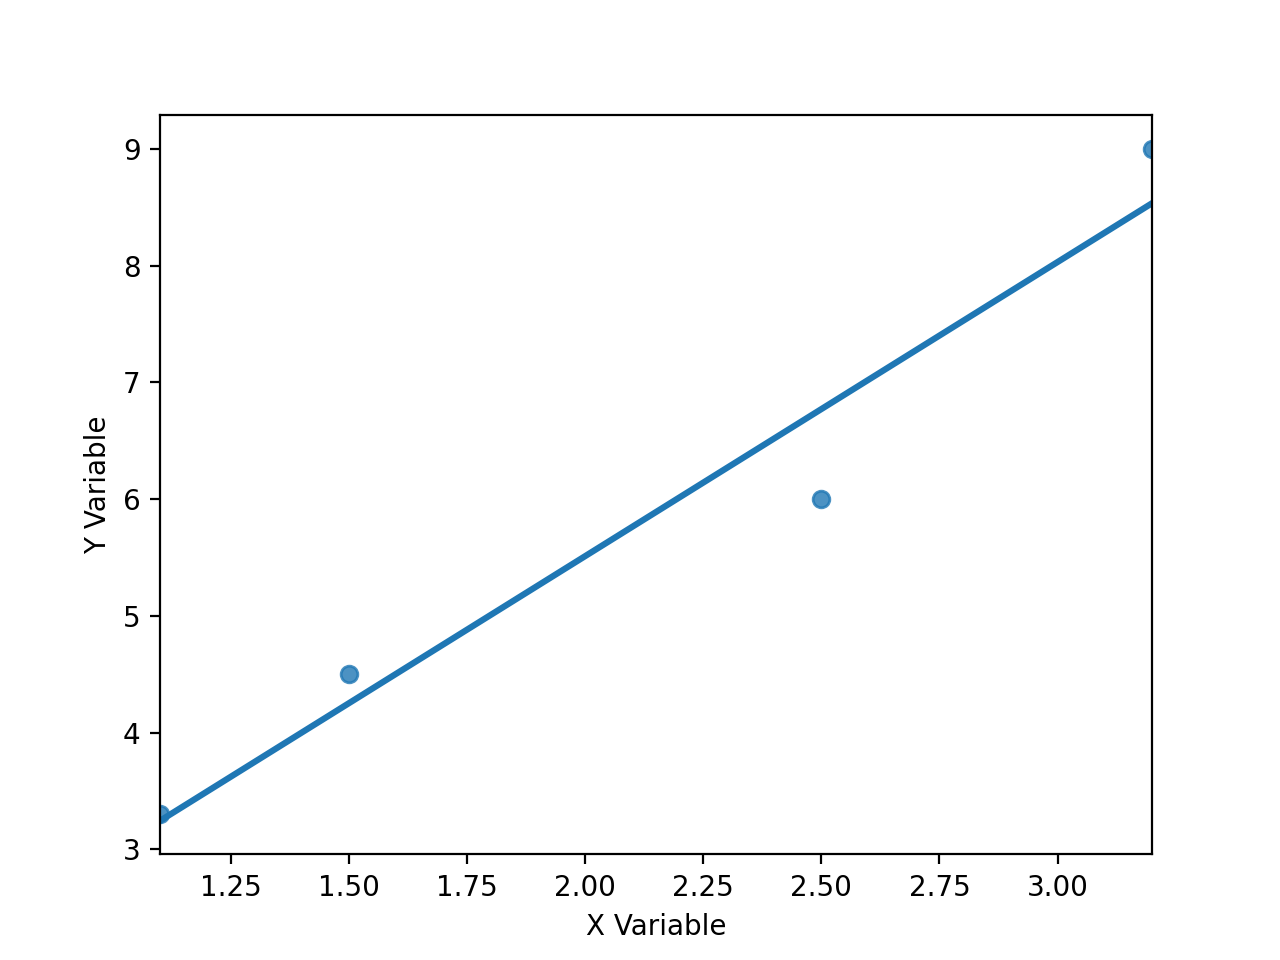
\includegraphics[width=0.7\textwidth]{mathematics/fig/linearRegressionExact.png}}

\subsubsection{$\boldsymbol{\chi}^2$ Minimization}
If each measurement is not made equally well for all points in the data set, the loss function can be adjusted to accommodate each individual measurements uncertainty. The $\chi^2$ of the fit is then used as the loss function, defined as
 \begin{align}
    	\chi^2 = \sum_{i=1}^N\Big(\frac{\B{wx}_i +b - y_i}{\sigma_i}\Big)^2
\end{align}
Where $\sigma_i$ is the uncertainty on the measured value $y_i$. An optimizer then looks to minimize this quantity
\begin{align}
    \min_\B{w}  \sum_{i=1}^N\Big(\frac{\B{wx}_i +b - y_i}{\sigma_i}\Big)^2
\end{align}


\subsubsection{Ridge Regression}
Ridge regression is a linear regression with an added penalty term proportional to the sum of the squared weights. If we have $M$ total features, then we can express each break up our weight vector $\B{w}$ into individual components as  $w_j$ for $j\in (1,M)$. For simplicity we will also take $w_0 = b$. Ridge regression therefore use the loss function defined below
\begin{align}
    	\min_\B{w} \Big[\alpha\sum_{j=0}^Mw_j^2 + \sum_{i=1}^N\Big(\B{wx}_i +b - y_i\Big)^2 \Big]
\end{align}
Ridge regression looks to prevent any one weight $w_j$ from becoming significantly larger than the rest due to the squaring. This effectively prevents the model from becoming heavily dependent on any single weight which is helpful in situations where the feature vectors are correlated (multicollinearity). 

Ridge regression is also preferred in some cases due to its differentiability, which allows it to be optimized using gradient descent.

\subsubsection{Lasso}
The LASSO (Least Absolute Shrinkage and Selection Operator) is defined as 

\begin{align}
    	\min_\B{w} \Big[\alpha\sum_{j=0}^M|w_j| + \sum_{i=1}^N\Big(\B{wx}_i +b - y_i\Big)^2 \Big]
    	\end{align}
    	
With $w_j$ in our $\B{w}$ vector for $j\in (1,M)$ and $w_0 = b$. It is similar in appearance to Ridge regression, although each weight is no longer squared. This  allows for the individual weights to go to zero (unlike Ridge Regression) and effectively selects for the smallest number of applicable weights. This is helpful if we want to reduce the number of parameters our model is dependent on.


\subsection{Gradient Descent}\label{grad-descent}

The gradient is the localized slope of a function. Gradient descent is a means of finding a minimum (typically of a loss function) by following this slope towards a minimum. The crux of gradient descent goes like this
\begin{enumerate}
    \item Initialize each of our weights $w_j$
    \item Begin a new \B{epoch} for which we use the entire dataset to calculate our error function $\mathcal{E}$ using our current weights $w_j$
    \begin{itemize}
    \item If this loss is below a threshold, we're done, otherwise we continue    
    \end{itemize}
    \item Calculate the gradient of our error function 
    \begin{align}
        \frac{\partial \mathcal{E}}{\partial w_j}
    \end{align}
    \item Move the weights in a direction such that the loss function should shrink by an amount proportional to the \B{learning rate} $\alpha$
    \begin{align}
        w_j \leftarrow w_j - \alpha\frac{\partial \mathcal{E}}{\partial w_j}
    \end{align}
    \item Loop back to Step 2.
\end{enumerate}

\subsubsection{Linear Regression with Gradient Descent}

 As an example, we have already calculated the gradient of our linear regression model in Section \ref{lin-reg-exact}. The gradient of the sum of squared errors is given by
\begin{align}
    \frac{\partial \mathcal{E}}{\partial w} &= 2\Big(w\sum_ix_i^2 + b\sum_i x_i -\sum_i y_i x_i\Big)\label{grad_sse_w}\\
    \frac{\partial \mathcal{E}}{\partial b} &= 2\Big(bN + w \sum_i x_i - \sum_i y_i \Big)\label{grad_sse_b}
\end{align}
Although we were able to solve this method exactly with some algebra before, it is instructive to show how gradient descent can be used on the same model, since in general it can be used in cases were we \emph{do not} have an exact solution.

Below shows the implementation of the algorithm described in Section \ref{grad-descent} for the same set of data as was used in the exact case.

\lstinputlisting[language=Python]{mathematics/code/linearRegressionGradient.py}

\centerline{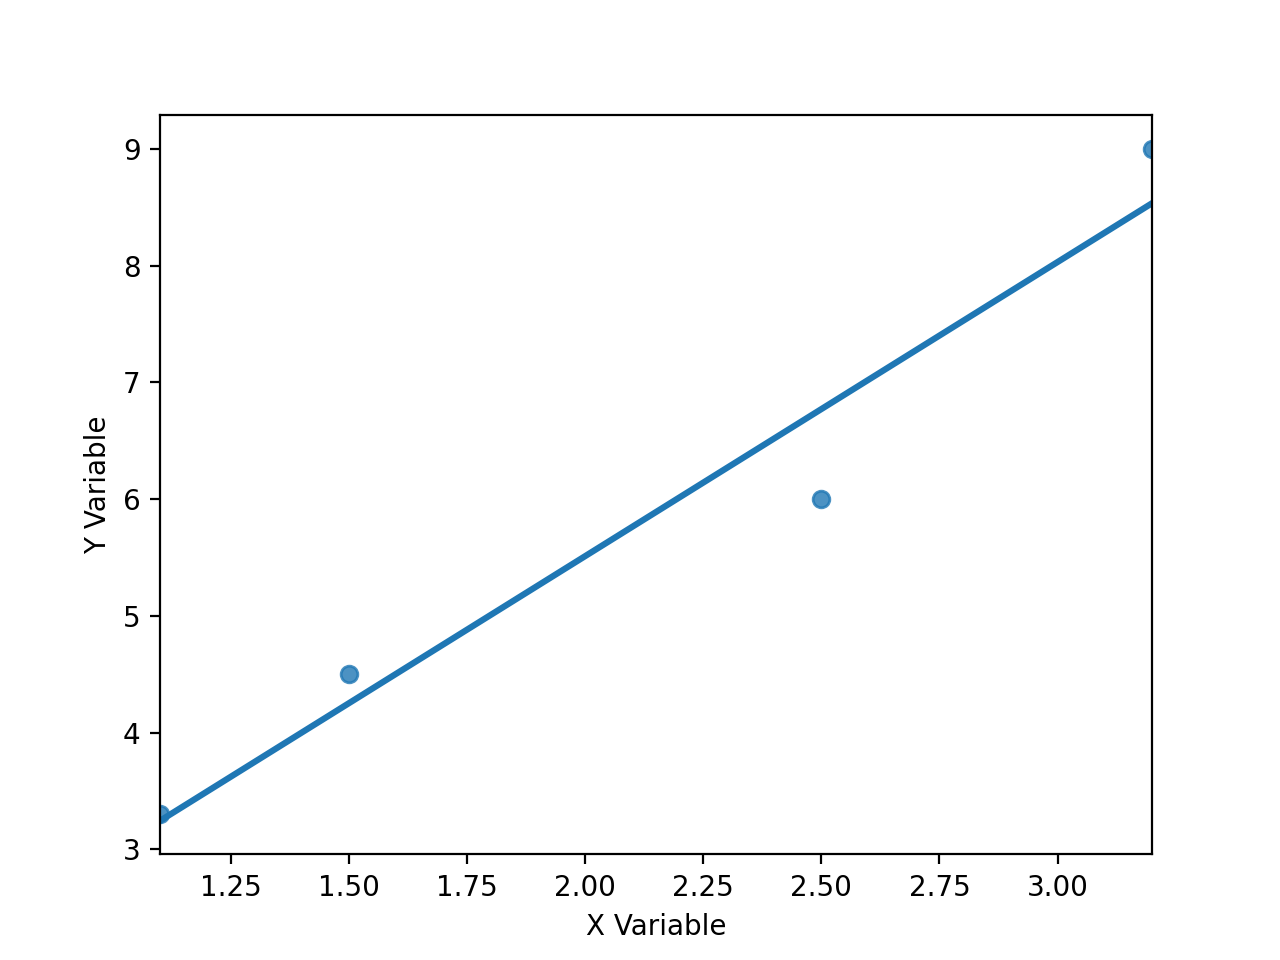
\includegraphics[width=0.7\textwidth]{mathematics/fig/linearRegressionGradient.png}}



\subsubsection{Minibatch and Stochastic Gradient Descent}

Gradient descent is powerful in its generality but can be rather slow since it requires looping over the entire dataset once for each epoch. This issue can be mitigated using one (or both) of the methods below
\begin{itemize}
    \item \B{Minibatch Gradient Descent}: Chops up the dataset into shuffled ``minibatches" for which gradients are calculated and the weights are adjusted within each epoch
    \item \B{Stochastic Gradient Descent}: Adjusts the weights based off of \emph{every data point} within each epoch. It is particularly useful when there is redundancy in the data and the gradient is stable.
\end{itemize}


\subsection{Newton's Method}
Newton's method uses the second order Taylor expansion of the function to estimate the extremum in an optimization problem. This is contrasted with gradient descent which uses only the first order. Given a point $x_k$ where the optimizer is currently while looking for the extremum of $f(x)$, we have that
\begin{align}
	f(x_k+t)\approx f(x_k) + f'(x_k)t + \frac{1}{2}f''(x_k)t^2
\end{align}
If the second derivative $f''(x_k)$ is positive, the extremum of $f(x_k+t)$ will be when $f'(x_k+t) = d/dt f(x_k+t) = 0$ since $x=x_k+t$. This can be written as 
\begin{align}
	\frac{d}{dt}\Big( f(x_k) + f'(x_k)t + \frac{1}{2}f''(x_k)t^2\Big) = f'(x_k)+f''(x_k)t = 0 
\end{align}
Therefore under these conditions, $t = -f'(x_k)/f''(x_k)$ and the we assign the best estimate for the extremum of the function as
\begin{align}
	f(x_{k+1}) = f(x_k)-\frac{f'(x_k)}{f''(x_k)}
\end{align} 


\subsection{$k$-Nearest Neighbors}\label{sub:knn}
One of the simpler machine learning algorithms, $k$-nearest neighbors (KNN) takes in a new event (with it's own set of features) and finds the  $k$ events in the training data which it is closest to. This distance definition is adjustable. Once all the neighbors have been found, each votes on how to classify the new event.

This distance metric generally scales exponentially when new dimension are introduced, so it is advised to run dimensionality reduction (Section \ref{dim_red}) if using KNN for a high dimensional dataset.
\subsection{Naive Bayes}
When trying to deduce the probability of something dependent on many features $X_i$ conditional on something $S$, the naive way to do it is to assume they are all independent of each other
\begin{align}\label{naive_bayes}
	P(X_1,X_2,\dots,X_n|S) = P(X_1|S)P(X_2|S)\dots P(X_n|S)
\end{align}
This is the assumption made in Naive Bayes, for which computing the right side of Equation \ref{naive_bayes} is much easier than when one would need to look out for correlations.

When estimating $P(X_i|S)$ it is typical to use a \textit{pseudocount} for it's estimate so we don't assign 0 or 1 to the probability and bias our results. According to \cite{sutton} this is
\begin{align}
	P(X_i|S) = (k+\textrm{number~of~} S's\textrm{~with~} X_i's) / (2k+\textrm{number~of~} S \textrm{~total})
\end{align}

\subsection{Cross-Validation}
Cross-validation is helpful in cases where you do not have enough data to split into the training-validation-test sets \cite{burkov}. The procedure creates effective validation regions as follows

\begin{enumerate}
    \item Fix the values of the hyperparameters you want to evaluate
    \item Split your training set into several subsets of the same size (each called a \B{fold}). Typically five-fold cross-validation is what is done e.g $\{F_1, F_2, \ldots, F_5\}$
    \item Train the same number of models as you have folds. Each model $f_i$ should be trained using each fold $F_j$ except for $F_{j=i}$. In our example model $f_1$ would use $\{F_2, F_3, F_4,F_5\}$
    \item Use the remaining fold $F_{j=i}$ as a validation region for each model $f_i$
    \item Assign the average value of the metric of interest you are looking at as the final value
\end{enumerate}
Grid search and cross-validation are sometimes used together to find the best values of hyperparameters for a given model.

%\subsection{Learning Rate}
%TODO
%
%\subsection{Step Size}
%When iterating through a machine learning algorithm, the "step-size" determines how quickly you change your state from where you start from. The way of doing this is somewhat of an art, with a multitude of options such as 
%\begin{itemize}
%	\item Constant step size
%	\item Step size which decreases as you make more iterations
%\end{itemize}
%\todo{ Add examples in \cite{sutton} with Reinforcement learning step sizes.}

%\subsection{Loss Functions}
%TODO
%\subsubsection{Sum of Squared Residuals}
%TODO

\subsection{Ant Colony Optimization}
TODO

\subsection{Dealing with Missing Features}
If the dataset you have contains entries for which some of the features are missing, the easiest thing to do is remove them from the dataset and proceed with the learning algorithm. If not, one option is to use \B{data imputation} which replaces the missing value be an average value over the dataset.


\section{Fitting Models}

A machine learning model is said to \B{underfit} the data if the model makes many mistakes on the training data. For example if a linear function is fit to set of features that change quadratically. A model that underfits its training data is said to have \B{high bias}, in that its expected value is know to differ from the true underlying distribution being estimated.

On the other hand, a model is said to \B{overfit} the data if the model fits the training data very well, but is seen to perform poorly on validation or test datasets. Models which overfit the data are said to have \B{high variance}, meaning small changes in your training data produce big changes to your model.

\subsection{Regularization}
Regularization is an umbrella term that encompasses a collection of methods that are used to decrease the complexity of models that machine learning algorithms produce.


Dropout: TODO
Batch-Normalization: TODO

\subsection{Model-Based vs Instance-Based Learning}
Model-based learning involves finding optimal parameters and uses a training dataset for its construction. An example is Support Vector Machines (Section \ref{sub:svm}). Model-based architectures typically construct three different datasets
\begin{itemize}
    \item \B{Training Dataset}: used to train the model
    \item \B{Validation Dataset}: used choose the best algorithm and  for tuning the hyperparameters 
    \item \B{Test Dataset}: Assesses the model before it is deployed in the wild
\end{itemize}

Instance-based learning involves using the whole dataset as the model. An example is $k$-Nearest Neighbors (Section \ref{sub:knn}).




\section{Classification}
Classification attempts to group like items together. In machine learning, a classification model attempts to ascribe a label given a set of features (e.g. ``spam", or ``not spam"). The performance breakdown of classifiers generally involves combinations of the following quantities

\begin{center}
 \begin{tabular}{||c c||} 
 \hline
\B{Name} (Abbr.) & \B{Description} \\ [0.5ex] 
 \hline\hline
Positive (P) & Real positive cases in the data  \\ 
 \hline
 Negative (N)& Real negative cases in the data  \\
 \hline
 True Positive (TP) & Positive cases correctly identified  \\
 \hline
True Negative (TN) & Negative cases correctly identified \\
 \hline
False Positive (FP) & Positive cases incorrectly identified   \\ 
 \hline
 False Negative (FN) &   Negative cases incorrectly identified\\
 \hline
\end{tabular}\label{forcing}
\end{center}

Another helpful breakdown of the table considers the total positive (P) and negative (N) cases in terms of those in the table
\begin{align}
    \textrm{P} = \textrm{TP+FN} && \textrm{N} = \textrm{TN+FP} 
\end{align}

\subsection{Accuracy}
A tests accuracy tells you how often you get the right answer, defined as
\begin{align}
	\textrm{Accuracy} = \frac{\textrm{TP+TN}}{\textrm{P+N}}
\end{align}

When writing a classifier, the accuracy of the model is not all that counts. For instance one can quite simply build a model that predicts with over $98\%$ accuracy if a newborn baby will ever develop leukemia. This model just predicts that no baby will develop leukemia, and is clearly not the kind of model that makes machine learning interesting.

\subsection{Confusion Matrix} 
 
 The confusion matrix (sometimes called the error matrix) is a tool used to visualize a classifiers performance which compares the label the algorithm predicted, and what it actually is.
\\
\\
\centerline{\begin{tabular}{cc|c|c|}
\cline{3-4}
 && \multicolumn{2}{ c| }{\B{Actual Value}} \\ \cline{3-4}
 && True & False  \\ \cline{1-4}
\multicolumn{1}{ |c  }{\multirow{2}{*}{\B{Predicted}}} &
\multicolumn{1}{ |c| }{True} & TP & FP       \\ \cline{2-4}
\multicolumn{1}{ |c  }{}                        &
\multicolumn{1}{ |c| }{False} & FN & TN     \\ \cline{1-4}
\end{tabular}}
\\

From these values we can measure the precision and recall which are both standard ways of measuring a classifiers performance. \B{Precision} is defined as
\begin{align}
	\textrm{Precision} = \frac{\textrm{TP}}{\textrm{TP+FP}}
\end{align}
which tells us the correct positive predictions to the total positive predictions. Another important quantity is the \B{recall} (sometimes called the sensitivity) which is defined as
\begin{align}
	\textrm{Recall} = \frac{\textrm{TP}}{\textrm{TP+FN}}
\end{align}

which tells us the correct positive predictions out of the total positive true cases. Both tell us different things. In the case of spam detection, we generally want high precision (i.e. all of the things we label as spam are actually spam) and can afford lower recall (i.e. we don't have to mark every piece of spam as spam). Both should always be reported together. The classifier is perfect if both precision and recall are one.

\subsection{ROC Curve}
The ROC curve stands for "receiver operating characteristic" and originates from radar engineering. Each curve, such as those shown in Figure \ref{fig:roc-curve} characterize the performance of a classifier. Each curve shows the \B{true positive rate} (TPR) against the \B{false positive rate} (FPR) for a given classifier with
\begin{align}
    \textrm{TPR} \doteq \frac{\textrm{TP}}{\textrm{TP+FN}} && \textrm{FPR} \doteq \frac{\textrm{FP}}{\textrm{FP+TN}}
\end{align}
Classifiers are only good if they are better than a random choice. The diagonal line defines the curve $\textrm{TP}/\textrm{P} = \textrm{FP} /\textrm{N}$, which is to say that the proportion of positives the classifier selects among actual positive values is equal to the amount of positives you mistakenly select among all the negative values. A good classifier however will always find the proportion of positives among all positive values at a greater rate than it will find positives among the negative values. This equates to 
\begin{align}
        \textrm{TPR} \geq \textrm{FPR}
\end{align}
and equates to a curve to the left of the random classifier. In the ideal case
we get all our positive guesses correct, which equates to a point at the top left.

Different curves are compared using the area under the curve (AUC), with a higher value implies a better classifier. Areas range from $0$ to $1$.

\begin{figure}
\centerline{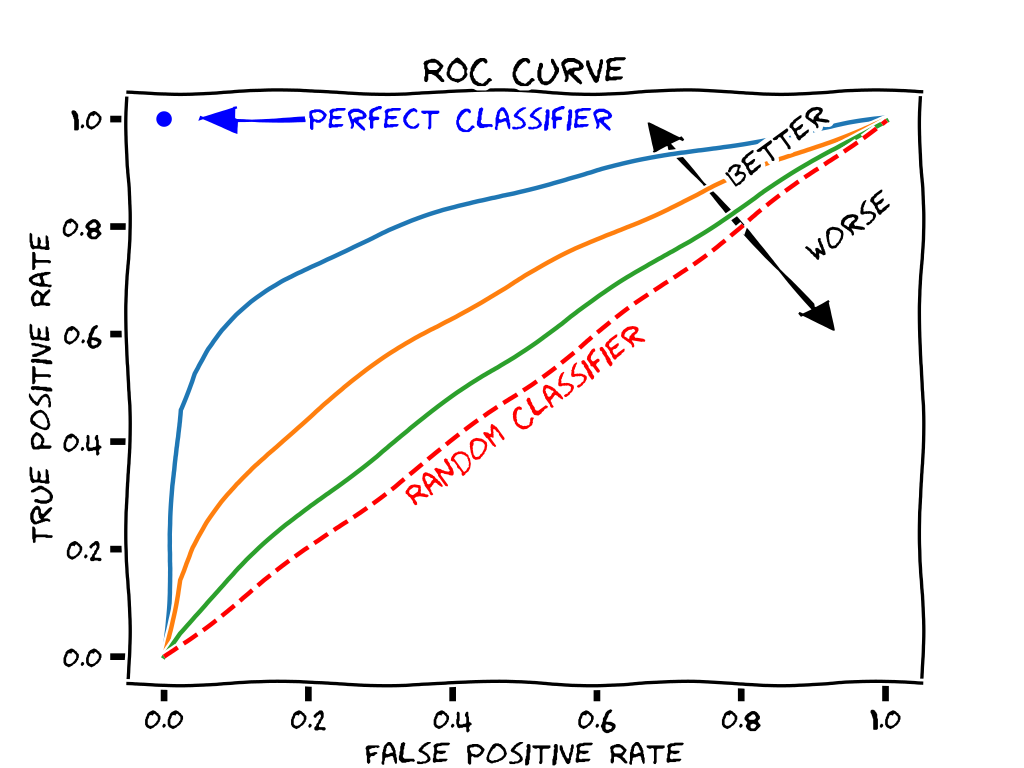
\includegraphics[width=0.7\textwidth]{mathematics/fig/rocCurve.png}}
\label{fig:roc-curve}
\caption{ROC curve}
\end{figure}

\subsection{Logisitic Regression}
Logistic regression is not in fact a regression but a classification algorithm. The idea is to parameterize how certain you are some set of features $\B{x}$ is, or is not within a certain class (i.e. $y\in \{0,1\}$). We do this via a function which outputs a value which corresponds to which class we think it is in. In essence we need a function with the properties
\begin{align}
    f(x)=1 &&\textrm{when}&~ x\rightarrow\infty\\
    f(x)=0 &&\textrm{when}&~ x\rightarrow-\infty
\end{align}
which is smooth (differentiable) in between. The class of these functions are known as \B{sigmoid functions}.  One example of a sigmoid function is the \B{logisitic function} which spans $(0,1)$ increasing monotonically with its argument.
\begin{align}
	f(x) = \frac{1}{1+e^{-x}}
\end{align}
This distribution is identical to the Fermi-Dirac distribution from Physics which describes the average number of fermions that occupy a given energy state. The logistic function also holds an attractive feature in its derivative
\begin{align}\label{eq:sig_der}
    \frac{d}{dx}f(x) = \frac{e^x\cdot(1+e^x)-e^x\cdot e^x}{(1+e^x)^2} = f(x)\Big(1-f(x)\Big)
\end{align}
Which allows for easy calculation of gradients. When doing machine learning typically a linear regression term is used for the exponent, to account for different dependencies of each feature.
\begin{align}
	f_{\mathbf{w},b}(\mathbf{x}) = \frac{1}{1+e^{-(\mathbf{wx} +b)}}
\end{align}
Where $\B{w}$ the weight vector and $b$ the offset are parameters to be fit. The optimal values for $\B{w}$ and $b$ are typically found via gradient descent. Following Equation \ref{eq:sig_der}, each parameter would be updated with the rule
\begin{align}
    \B{w}&\leftarrow\B{w}+\alpha~\B{x} f_{\mathbf{w},b}(\mathbf{x}) \Big(1-f_{\mathbf{w},b}(\mathbf{x})\Big)\\
    b&\leftarrow b +\alpha f_{\mathbf{w},b}(\mathbf{x}) \Big(1-f_{\mathbf{w},b}(\mathbf{x})\Big)
\end{align}


\subsubsection{Softmax Function}
The softmax function is the multinomial version of the logisitic function, used for when we have more than two categories. It is defined as 
\begin{align}
    \sigma(x_i) = \frac{e^{x_i}}{\sum_{j=1}^K e^{x_j}}
\end{align}
Where $K$ is the total amount of categories you have and $i\in(1,\ldots,K)$. For each category $i$, some real-valued quantity $x_i\in(-\infty,\infty)$ is calculated from the objects features $\B{x}$. Those with features similar to a category have a large $x_i$, and those unlike the category yield a small $x_i$. The relative probability among the different categories is then given by $\sigma(x_i)$. The denominator is used to normalize the quantity to unity. The softmax function is identical to the Boltzmann distribution of Physics.



\section{Neural Networks}
The main ingredients in neural networks are units that perform logistic regression. Each of these units, which acts analogously to a neuron in the brain, are called a \B{perceptron}. These perceptrons are put in \B{layers} which generally feed the into one another. Each perceptron itself is a mathematical function which acts on its input via it's activation function $g$, and provides an output $y$

%
%\begin{figure}[t]
%	\centering
%	\begin{tikzpicture}[shorten >=1pt]
%		\tikzstyle{unit}=[draw,shape=circle,minimum size=1.cm]
% 		\tikzstyle{hidden}=[draw,shape=rectangle,minimum size=1.15cm]
%        \tikzstyle{annot_small} = [text width=4em, text centered]
%        \tikzstyle{annot_big} = [text width=8em, text centered]
%
%		\node[unit](x0) at (-2,3){$x_0$};
%		\node[unit](x1) at (-2,1){$x_1$};
% 
%		\node[hidden](h10) at (1.7,3.5){$y_0^{(1)}\leftarrow g^{(1)}(\B{w}_{1,0}\B{x}+b_{1,0})$};
%		\node[hidden](h11) at (1.7,2){$y_1^{(1)}\leftarrow g^{(1)}(\B{w}_{1,1}\B{x}+b_{1,1})$};
%		\node[hidden](h12) at (1.7,0.5){$y_2^{(1)}\leftarrow g^{(1)}(\B{w}_{1,2}\B{x}+b_{1,2})$};
% 
%		\node(h22) at (5,0){};
%		\node(h21) at (5,2){};
%		\node(h20) at (5,4){};
%		
%		\node[hidden](h20) at (7.5,3.5){$y_0^{(2)}\leftarrow g^{(2)}(\B{w}_{2,0}\B{y}^{(1)}+b_{2,0})$};
%		\node[hidden](h21) at (7.5,2){$y_1^{(2)}\leftarrow g^{(2)}(\B{w}_{2,1}\B{y}^{(1)}+b_{2,1})$};
%		\node[hidden](h22) at (7.5,0.5){$y_2^{(2)}\leftarrow g^{(2)}(\B{w}_{2,2}\B{y}^{(1)}+b_{2,2})$};
%		
%	
%		\node[unit](y1) at (11,2){$y$};
%		
%		\foreach \i in {0,...,1}
%		  \foreach \j in {0,...,2}
%		{
%		  \draw[->] (x\i) -- (h1\j.west);
%		}
%		
%		\foreach \i in {0,...,2}
%		  \foreach \j in {0,...,2}
%		{
%		  \draw[->] (h1\i.east) -- (h2\j.west);
%		}
% 
%		\foreach \i in {0,...,2}
%		{
%		  \draw[->] (h2\i.east) -- (y1);
%		}    
%        
%        \node[annot_small, above of=x0, node distance=1.5cm](input){input layer};
%        \node[annot_big, above of=h10, node distance=1.5cm](hide1){$1^{\textrm{st}}$ hidden layer};
%        \node[annot_big, above of=h20, node distance=1.5cm](hide2){$2^{\textrm{nd}}$ hidden layer};
%        \node[annot_small, above of=y1, node distance=2.cm](output){output layer};
%        
%        \end{tikzpicture}
%	\caption[mlp]{Two hidden-layer, feedforward neural network. Two features are feed into the first hidden layer with activation function $g^{(1)}$. The outputs of the first hidden layer $y^{(1)}$ are feed into the second layer with activation function $g^{(2)}$. The output of the second layer $y^{(2)}$ are then combined to form a single output.}
%	\label{fig:multilayer-perceptron}
%\end{figure}



\begin{figure}[t]
	\centering
	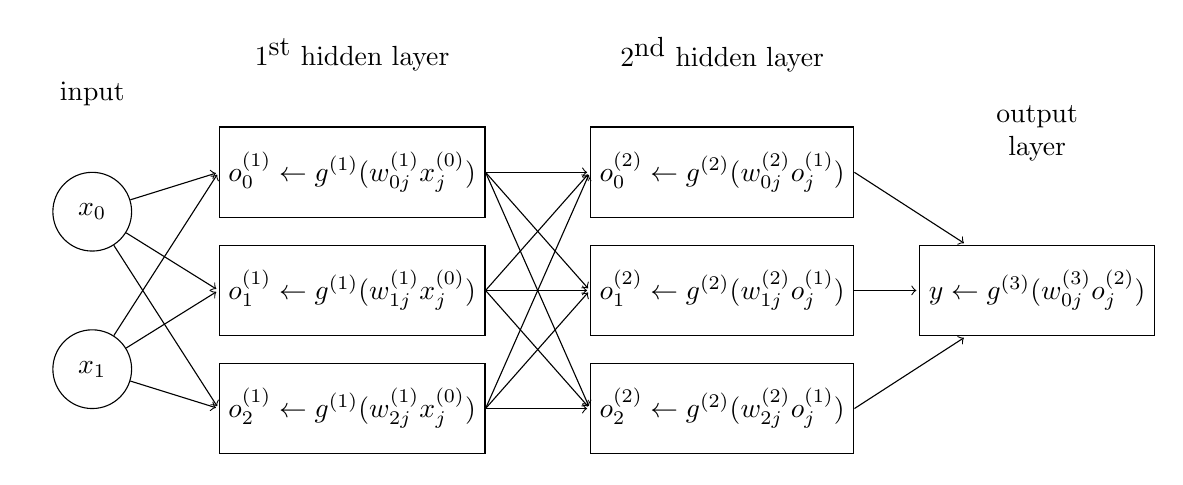
\begin{tikzpicture}[shorten >=1pt]
		\tikzstyle{unit}=[draw,shape=circle,minimum size=1.cm]
 		\tikzstyle{hidden}=[draw,shape=rectangle,minimum size=1.15cm]
        \tikzstyle{annot_small} = [text width=4em, text centered]
        \tikzstyle{annot_big} = [text width=8em, text centered]

		\node[unit](x0) at (-2,3){$x_0$};
		\node[unit](x1) at (-2,1){$x_1$};
 
		\node[hidden](h10) at (1.3,3.5){$o_0^{(1)}\leftarrow g^{(1)}(w_{0j}^{(1)}x_j^{(0)})$};
		\node[hidden](h11) at (1.3,2){$o_1^{(1)}\leftarrow g^{(1)}(w_{1j}^{(1)}x_j^{(0)})$};
		\node[hidden](h12) at (1.3,0.5){$o_2^{(1)}\leftarrow g^{(1)}(w_{2j}^{(1)}x_j^{(0)})$};
 
		\node(h22) at (5,0){};
		\node(h21) at (5,2){};
		\node(h20) at (5,4){};
		
		\node[hidden](h20) at (6.,3.5){$o_0^{(2)}\leftarrow g^{(2)}(w_{0j}^{(2)}o_j^{(1)})$};
		\node[hidden](h21) at (6.,2){$o_1^{(2)}\leftarrow g^{(2)}(w_{1j}^{(2)}o_j^{(1)})$};
		\node[hidden](h22) at (6.,0.5){$o_2^{(2)}\leftarrow g^{(2)}(w_{2j}^{(2)}o_j^{(1)})$};
		
	
		\node[hidden](y1) at (10,2){$y\leftarrow g^{(3)}(w_{0j}^{(3)}o_j^{(2)})$};
		
		\foreach \i in {0,...,1}
		  \foreach \j in {0,...,2}
		{
		  \draw[->] (x\i) -- (h1\j.west);
		}
		
		\foreach \i in {0,...,2}
		  \foreach \j in {0,...,2}
		{
		  \draw[->] (h1\i.east) -- (h2\j.west);
		}
 
		\foreach \i in {0,...,2}
		{
		  \draw[->] (h2\i.east) -- (y1);
		}    
        
        \node[annot_small, above of=x0, node distance=1.5cm](input){input};
        \node[annot_big, above of=h10, node distance=1.5cm](hide1){$1^{\textrm{st}}$ hidden layer};
        \node[annot_big, above of=h20, node distance=1.5cm](hide2){$2^{\textrm{nd}}$ hidden layer};
        \node[annot_small, above of=y1, node distance=2.cm](output){output layer};
        
        \end{tikzpicture}
	\caption[mlp]{Three layer feed-forward neural network with two hidden-layers. Two features are feed into the first hidden layer with activation function $g^{(1)}$. The outputs of the first hidden layer $o_j^{(1)}$ are feed into the second layer with activation function $g^{(2)}$. The output of the second layer $o_j^{(2)}$ are then feed into the output layer activation function $g^{(3)}$ and combined to form a single output.}
	\label{fig:multilayer-perceptron}
\end{figure}


Figure \ref{fig:multilayer-perceptron} shows a \B{multilayer perceptron} (MLP) neural network architecture. This network is \B{feed-forward} meaning that all perceptrons connect in the direction going from input to output. Each layer itself is \B{fully-connected}, meaning that each output the preceding layer is used as input for each of the nodes in the following layer.

\subsubsection{Notation}
List of terms used to describe an $m$ layer neural network are listed below\cite{brilliant_backpropagation}. Values in parentheses 
\\
\begin{tabular}{ l c }
  $r_l$ & number of neurons on layer $l\in[1,m]$\\
  $w_{ij}^{(l)}$ & weight given to output of neuron $j$ used in neuron $i$ on layer $l$  \\
  $b_i^{(l)}$ & bias used in neuron $i$ on layer $l$   \\
  $a_i^{(l)}$ & the product sum plus bias (activation) for node $i$ on layer $l$  \\
  $o_i^{(l)}$ & the output of neuron $i$ on layer $l$ \\
  $g^{(l)}$ & activation function for the hidden layer neurons\\
\end{tabular}\\
\\
Explicitly, the activation is written as
\begin{align}
	a_i^l =b_i^l + w_{ij}^lo_j^{l-1}
\end{align}
With summation implied following Einstein notation (Section \ref{einstein_notation}) and $j\in [1,r_{l-1}]$. If we define
\begin{align}
	w^l_{0i}=b_i^l && o_0^{l-1}=1
\end{align}
We can simplify the sum to
\begin{align}\label{nn_activation}
	a_i^l = w_{ij}^lo_j^{l-1}
\end{align}
with $j\in [0,r_{l-1}]$.

\subsubsection{Activation Functions}
The activation function $g$ of a neural network must be differentiable, but otherwise has no hard constraints. Some that are typically used:
\begin{itemize}
    \item \B{Logistic function}
\begin{align}
	g(x) = \frac{1}{1+e^{-x}}
\end{align}
Recently fallen out of favor since $g(0)=1/2$, which means a perceptron with input sum $0$ would have a positive output. Additionally the gradient is very small for large $|x|$, which leads to weights getting stuck \cite{grus}.
    \item \B{TanH}
\begin{align}
    g(x) = \tanh (x) = \frac{e^x-e^{-x}}{e^x+e^{-x}}
\end{align}
    Hyperbolic tangent is a popular alternative to the logistic function.
    \item \B{ReLU}
    \begin{align}
     g(x)= 
\begin{cases}
    0 & \text{if } x <  0\\
    x & \text{otherwise}
\end{cases}
\end{align}
The Rectified Linear Unit is popular because its derivative is so simple to calculate which allows neural networks with many layers to update more easily. Additionally it does not have a problem with a vanishing gradient explained in Section \ref{sec:backprop}, unlike both TanH and the Logistic function.
\end{itemize}

\subsection{Backpropagation}\label{sec:backprop}
To calculate the correct weights used by the activation function of each perceptron, typically some form of gradient descent is used in conjunction with an error function $\mathcal{E}$. This requires one to be able to compute the gradient of $\mathcal{E}$ with respect to the individual perceptrons weights. Using gradient descent, we look for
\begin{align}
\frac{\partial \mathcal{E}}{\partial w_{ij}^l}
\end{align}
Between the output and the weights themselves, a lot of manipulation goes on. Firstly the weights are combined in the activation product sum $a_i^l$ of layer $l$. Mathematically this lets us break up the derivative via the chain rule. 
\begin{align}\label{eq:nn_weight_chain_rule}
    \frac{\partial \mathcal{E}}{\partial w_{ij}^l} = \frac{\partial \mathcal{E}}{\partial a_i^l}\frac{\partial a_i^l}{\partial w_{ij}^l}
\end{align}
The second term is easily computed using Equation \ref{nn_activation} with
\begin{align}
	\frac{\partial a_{i}^l}{\partial w_{ij}^l} = o_j^{l-1}
\end{align}
The first term is usually called the \textbf{error}, defined as 
\begin{align}
	\delta_{i}^l \equiv \frac{\partial \mathcal{E}}{\partial a_{i}^l}
\end{align}
In general this term can be complicated since there are potentially many perceptron layers through which the activation $a_i^l$ must pass through before it eventually affects the final output and therefore the error function $\mathcal{E}$. One can most clearly arrive at an expression for $\delta^l_i$ by first considering the output layer, layer $m$, for which the expression is given as
\begin{align}\label{eq:error_out_lay}
	\delta_{i}^m \equiv \frac{\partial \mathcal{E}}{\partial a_{i}^m} &=  \frac{\partial \mathcal{E}}{\partial g^m} \frac{\partial g^m}{\partial a_{i}^m}
\end{align}
The first term is typically trivially computed; for example if the error function is SSE, then
\begin{align}\label{eq:error_out_lay_1}
    \frac{\partial \mathcal{E}}{\partial g^m} = \frac{\partial }{\partial g^m}\sum_{p=0}^N (g^m - y_p)^2 = \sum_{p=0}^N 2(g^m - y_p)
\end{align}
Where $p\in(1,\ldots,N)$ are the total number of data points you have. The second term of Equation \ref{eq:error_out_lay} is just the derivative of the activation function.
\begin{align}\label{eq:error_out_lay_2}
    \frac{\partial g^m}{\partial a_{i}^m} = g'^{~m}(a_{i}^m)
\end{align}
The activation function is typically chosen such that the derivative is either easily computed, or can be expressed in terms of the function itself (e.g. the logistic function). 

At this stage, we are capable of expressing the gradient with respect to the weights of the last layer. We simply plug in our current weight values into Equations \ref{eq:error_out_lay_1} and \ref{eq:error_out_lay_2} and then \ref{eq:nn_weight_chain_rule} we get a numerical expression for our gradient with respect to the weights. 



The reason why this method is called \textbf{backpropagation} is because the $\delta_i^m$ term from the last layer is then propagated backwards through the network to adjust weights in the other neurons. Let us next look for the change in layer $m-1$
\begin{align}
	\delta_j^{m-1} \equiv \frac{\partial \mathcal{E}}{\partial a_{j}^{m-1}} &= \frac{\partial \mathcal{E}}{\partial a_{i}^{m}}\frac{\partial a_{i}^{m}}{\partial a_{j}^{m-1}}
\end{align}
However we already have an expression for the first term, $\delta_i^m$! We also have the numerical value for this expression as well. This leaves us with only having to calculate the second term.
We can then recognize that the output of the previous layer is whatever its activation function spits out
\begin{align}
	o_j^{l-1} &= g^{l-1}(a_j^{l-1})
\end{align}
this then tells us that the activation fed into the last layer can be expressed as a function of the previous layers activation
\begin{align}
	a_i^m = w_{ij}^m g^{m-1}(a_j^{m-1})
\end{align}
And thus we have a recursive relation with
\begin{align}
	\delta_j^{l-1} = \delta_i^l w_{ij}^l g'^{~l-1}(a_j^{l-1})
\end{align}
Which gives us the gradient for an arbitrary hidden layer  after starting from the output layer
\begin{align}
	\frac{\partial \mathcal{E}}{\partial w_{ij}^l} = \delta_j^{l}o_i^{l-1} = \delta_n^{l+1} w_{nj}^{l+1} g'^{~l}(a_j^{l})o_j^{l-1}
\end{align}
The weights are then adjusted using gradient descent with
\begin{align}
	\Delta w_{ij}^l = -\alpha~  \frac{\partial \mathcal{E}}{\partial w_{ij}^l}
\end{align}
The issue with the chain rule being applied so many times is that one can run into a \B{vanishing gradient}. Using ReLU activation functions is one method of fixing this. The problem of an  \B{exploding gradient} can be solved by regularizing the loss function (e.g. hinge or LASSO).
%
%\subsection{Feed Forward Networks}
%A feed forward neural network (FFNN) only has neurons which take inputs from the previous layer and pass them to the next layer. Consider $m$ total layers and the following definitions \cite{brilliant_backpropagation}
%\\
%\begin{tabular}{ l c }
%  $r_k$ & number of neurons on layer $k\in[1,m]$\\
%  $w_{ij}^k$ & weight given to output of neuron $j$ used in neuron $i$ on layer $k$  \\
%  $b_i^k$ & bias used in neuron $i$ on layer $k$   \\
%  $a_i^k$ & the product sum plus bias (activation) for node $i$ on layer $k$  \\
%  $o_i^k$ & the output of neuron $i$ on layer $k$ \\
%  $g$ & activation function for the hidden layer neurons \\
%  $g_o$ & activation function for the output layer neurons \\
%\end{tabular}\\
%\\
%Explicitly, the activation is written as
%\begin{align}
%	a_i^k =b_i^k + w_{ij}^ko_j^{k-1}
%\end{align}
%With summation implied following Einstein notation (Section \ref{einstein_notation}) and $j\in [1,r_{k-1}]$. If we defined 
%\begin{align}
%	w^k_{0i}=b_i^k && o_0^{k-1}=1
%\end{align}
%We can simplify the sum with
%\begin{align}\label{nn_activation}
%	a_i^k = w_{ij}^ko_j^{k-1}
%\end{align}
%with $j\in [0,r_{k-1}]$.
%

\subsection{Convolutional Neural Networks}

As one continues to add more parameters to a fully connected feed forward network, each additional hidden layer increases the number of parameters by $(r_{l-1}+1)\cdot r_l$. This can be seen picturing each neuron $r_l$ which has a weight for each connection to the previous layer $r_{l-1}$ and  plus an offset. Convolutional neural networks (CNN) reduce the number of parameters that you need by using convolutional windows which generalize patterns in the data. CNN were initially developed for image recognition but nowadays are also used in text processing. 

Imagine you are looking for a feature in an image that is a sloping diagonal line. A \textbf{filter} for that image may look like
\begin{align}
    \textbf{F} = 
\begin{pmatrix}
0 & 0 & 1 \\
0 & 1 & 0 \\
1 & 0 & 0
\end{pmatrix}
\end{align}
The filter itself is \emph{learned} just as how weights are learned in a standard FFNN, with each matrix element being a parameter that is optimized for.

Let us now imagine the photo we want to recognize, which is an matrix of integers corresponding to the color intensity. Lets imagine we have a grayscale image, which happens to be the size of our filter.
\begin{align}
    \textbf{I} = 
\begin{pmatrix}
0 & 2 & 5 \\
9 & 7 & 0 \\
1 & 2 & 9
\end{pmatrix}
\end{align}
The \textbf{convolution} of the two is defined as
\begin{align}
\textbf{F} * \textbf{I} = 
\begin{pmatrix}
0 & 0 & 1 \\
0 & 1 & 0 \\
1 & 0 & 0
\end{pmatrix}
*
    \begin{pmatrix}
0 & 2 & 5 \\
9 & 7 & 0 \\
1 & 2 & 9
\end{pmatrix}
=     
\begin{pmatrix}
0\cdot 0 & 0\cdot2 & 1\cdot 5 \\
0\cdot 9 & 1\cdot 7 & 0\cdot 0 \\
1\cdot 1 & 0\cdot 2 & 0 \cdot 9
\end{pmatrix} = 13
\end{align}
We can recognize that the filter shrinks down the output that is fed into the next layer, we start here with a $3\times 3$ image which is filtered by a $3\times 3$ filter, leading to a single output. If we hitched another layer at the end of the filter layer, it would therefore have only \emph{one} input, whereas in a standard FFNN, we would have the same as the input.

Of course we often want to scan images for features smaller than their size. In this typical case the convolution is calculated using a scanning window, and is calculated everywhere it can fit. This operation results in a matrix smaller than the original input size. How to interact with the edge of the image is determined by \textbf{padding} which places arrays of zeroes on the edges of the image such that the convolution can be calculated outside the body of the image. One can also set the \textbf{stride} which determines how many pixels the filter skips over when moving to the next window.

To decrease the training time and the number of parameters needed in the model, \textbf{pooling} is often used as an alternative to trainable filters. Generally the windows have either their $\max$ or $\textrm{average}$ calculated instead of a convolution with a filter. Both are pooling and convolution are often used together, with a pooling layer typically following a convolutional layer.


\subsection{Recurrent Neural Networks}
Recurrent neural networks are used to label, classify, or generate sequences.

TODO



 A convolutional neural network (CNN) is a special kind of FFNN network that significantly reduces the number of parameters in a neural network without losing quality of the model. CNNs were initially developed with image and text processing in mind.


\subsection{Activation Functions}
% TODO Tanh, ReLU, Sigmoid, ...
ReLU fixes the problem of vanishing gradient




\subsection{Long-Short Term Memory (LSTM) Networks}
% TODO Long-Short Term Memory

\subsection{Encoders and Decoders}
Take two different sequences of data, for instance an English sentence composed of words $x_i$ with $i\in (1,N)$ and it's corresponding translation into French words $y_j$ with $j\in(1,M)$.

The encoder transforms the input sequence of words $x_i$ into something called a context vector (e.g. One-Hot encoding). Context vector is then feed to the decoder, which uses the context vector together with the previously generated symbol of the output sequence. 

\subsubsection{One-Hot Encoding}
One way to convert categorical data into learnable features is by using one-hot encoding. This method converts each category into an index in an array. For instance if we have three categories (red, green, blue), we can represent these as
\begin{align}
    \textrm{red} &= [1,0,0]\\
    \textrm{green} &= [0,1,0]\\
    \textrm{blue} &= [0,0,1]
\end{align}


The location of each category can then be used as a feature which can be learned.

\subsection{Attention}

The general idea here is the colloquial usage of attention, where you have to choose what things to pay attention to. Deep nets generally react more strongly to parts of the data than others which is effectively the network selecting what it should pay attention to (e.g. the network may look at spots to look for a leopard over a jaguar).



From Wikipedia: ``In the context of neural networks, attention is a technique that mimics cognitive attention. The effect enhances the important parts of the input data and fades out the rest -- the thought being that the network should devote more computing power on that small but important part of the data. Which part of the data is more important than others depends on the context and is learned through training data by gradient descent. "


\subsection{Transformers}
TODO

\url{https://jalammar.github.io/illustrated-transformer/}\\
\url{https://wiki.pathmind.com/attention-mechanism-memory-network}

\section{Dimensionality Reduction}\label{dim_red}
When fitting to a high dimensional space, the model can become overfit and/or the correlation within the feature vectors can be overlooked. In order to reduce the feature vectors into a space which has more discriminating power, it is helpful to reduce the total dimensions of the problem at hand.
\subsection{Principal Component Analysis (PCA)}
Principal Component Analysis (PCA) turns our feature space into ``Principal Components", eigenvectors of our individual features. The analysis finds the dimension in the data that contains the most variance, thereby having the most discriminating power between events.

We first begin with our feature vectors
$$\mathbf{X} = \left.\left( 
                  \vphantom{\begin{array}{c}1\\1\\1\\1\\1\end{array}}
                  \smash{\underbrace{
                      \begin{array}{ccccc}
                             x_{00}&x_{10}&x_{20}&\cdots &x_{p0}\\
                             x_{01}&x_{11}&x_{21}&\cdots &x_{p1}\\
                             x_{02}&x_{12}&x_{22}&\cdots &x_{p2}\\
                             \vdots&&&\ddots&\\
                             x_{0n}&x_{1n}&x_{2n}&\cdots &x_{pn}
                      \end{array}
                      }_{p\text{ features}}}
              \right)\right\}
              \,n\text{ events}
$$\\

The idea is to shrink the dimensionality, so change $p\rightarrow l$ where $l$ is the desired dimensionality after PCA. 

We first start by normalizing each feature $k=1,\dots,p$ to have $\mu=0$ (centers the data) and $\sigma=1$ (accounts for different units).

\begin{align}
\mu_k = \frac{1}{n}\sum_{j=1}^n x_{kj} && \sigma_k^2 = \frac{1}{n-1}\sum_{j=1}^n (x_{kj}-\mu_k)^2 \\
\end{align}
It is worth noting the definition used by $\texttt{scikitlearn}$ only normalizes the mean, but not the standard deviation of each feature. We then redefine each column $k$ in the matrix with
\begin{align}
	\rho_{kj} = (x_{kj} - \mu_k)/\sigma_k
\end{align}
This gives us a new matrix
$$\mathbf{\tilde{X}} =  \left.\left( 
                  \vphantom{\begin{array}{c}1\\1\\1\\1\\1\end{array}}
                  \smash{\underbrace{
                      \begin{array}{ccccc}
                             \rho_{00}&\rho_{10}&\rho_{20}&\cdots &\rho_{p0}\\
                             \rho_{01}&\rho_{11}&\rho_{21}&\cdots &\rho_{p1}\\
                             \rho_{02}&\rho_{12}&\rho_{22}&\cdots &\rho_{p2}\\
                             \vdots&&&\ddots&\\
                             \rho_{0n}&\rho_{1n}&\rho_{2n}&\cdots &\rho_{pn}
                      \end{array}
                      }_{p\text{ features}}}
              \right)\right\}
              \,n\text{ events}
$$\\

Now we look at the Covariance matrix (Section \ref{covmat}) of each of our $p$ features, with
\begin{align}
\textbf{K}_{\rho_i,\rho_j} = \begin{pmatrix} 
                             \Cov[\rho_0,\rho_0]&\Cov[\rho_1,\rho_0]&\cdots &\Cov[\rho_p,\rho_0]\\
                             \Cov[\rho_0,\rho_1]&\Cov[\rho_1,\rho_1]&\cdots &\Cov[\rho_p,\rho_1]\\
                             \vdots&\vdots&\ddots&\vdots\\
                             \Cov[\rho_0,\rho_p]&\Cov[\rho_1,\rho_p]&\cdots &\Cov[\rho_p,\rho_p] \end{pmatrix}
\end{align}
This matrix will be symmetric, with $1$ along the diagonal (since we scale each feature to have a variance of 1). The next step is to diagonalize this matrix following Section \ref{diagonalize} and find it's eigenvalues $\lambda_i$ and eigenvectors $\textbf{a}_i = a_{ik}$. This puts the matrix into the form

$$\bf{K}' = \left(
{\begin{array}{cccc}
\lambda_0 & 0 &...&0 \\
0 & \lambda_1 & ...&0\\
\vdots & \vdots &\ddots & \vdots \\
0 & 0 & ... &\lambda_p
\end{array}}
\right)
$$

One can recognize now that in our new coordinate system, we have a new set of variables which each have a variance represented by the eigenvalue $\lambda_i$ itself. Because we want the most discriminating variable, we sort the eigenvectors and eigenvalues by the largest $\lambda_i$, which corresponds to the largest variance. Our new feature space is therefore
\begin{align}
	\rho_{ij} = a_{ik}\rho_{kj}
\end{align}
With $i=1,\dots,l$.


\section{Reinforcement Learning}
Reinforcement learning aims to try to maximize some numerical reward signal. The most important distinguishing feature is that it uses training information to evaluate actions taken rather than instruct which action to take \cite{sutton}.


\subsection{$k$-armed Bandits}
Slot machines are sometimes called "one-armed bandits" for the single lever they have together with their ability to steal money from peoples pockets. The idea behind $k$-armed bandits is to imagine instead of a single slot machine, you have $k$ of them. Each machine has a probability distribution of for hitting the "jackpot", and your job is to find out which one gives you the highest payoff.

Searching for the highest value machine involves a trade-off between $exploiting$ the information you have now and $exploring$ the space to look for something better you haven't found yet.

Greedy algorithms, in this case, use the lever which currently has the highest estimated chance of success. $\epsilon$-greedy algorithms do the same thing, but one in $\epsilon$ times, will select one of the levers at random instead to explore.


\subsubsection{Upper-Confidence-Bound Action Selection}

One can also use confidence bounds on the unknown probabilities to determine which lever to pull next. Because we don't want to miss out on a lever which could potentially be higher than the one we currently see is highest, we use the upper-confidence-bound when picking our current highest value estimate. To find the relevant confidence interval, we start with Hoeffding's Inequality (Section \ref{hoeffding}), which eventually tells us
\begin{align}
	A_t = \textrm{argmax}\Big[Q_t(a) + c\sqrt{\frac{\ln t}{N_t(a)}}\Big]
\end{align}
Where $A_t$ is the next action taken at time $t$ (i.e. iterations through the algorithm). $Q_t(a)$ is the expected value of action $a$ at time $t$. $c$ is the confidence level. $N_t(a)$ is the amount of times $a$ has been tried.

Overall, this tells us if an action $a$ is tried many times, $N_t(a)$ gets larger and the bound shrinks. Meanwhile, as time goes on, the bound itself grows to represent uncertainty in the system itself as to if it changes with time.


\subsection{Markov Decision Processes}
Markov Decision Processes (MDP) concerns using probability to optimize movement between "states". The framework proposes that the learning problem can be broken down into three signals that are passed back and forth: 
\begin{enumerate}
	\item Actions $A$
	\item States $S$
	\item Rewards $R$
\end{enumerate}
At present, how to represent states and actions is more of an art than a science \cite{sutton}. Rewards however are simple single numbers.


\section{Modern Developments}
The machine learning field is quickly evolving with lots of terminology that is easy to forget. Here is a collection of terms and ideas on the forefront of the field.


\subsection{Metrics}
Different metrics are used to gauge the performance of a machine learning model

BLEU: bilingual evaluation understudy (used for evaluating language translation tasks).

